\chapter{Semi-supervised Learning}
\label{chap:SemisupervisedLearning}

This chapter provides an overview of semi-supervised learning (SSL). The following text draws information predominantly from the article \emph{An Overview of Deep Semi-Supervised Learning} (\cite{SemisupervisedOverview}) and from the book \emph{Semi-supervised learning} (\cite{SslBook}).

In deep learning, the goal typically is to learn some function $f: X \rightarrow Y$ by training a neural network on pairs of data points $(x, y)$. Deep neural networks have large number of trainable parameters, which require adequately large training datasets. Not having enough training data causes the model to overfit and then be unable to generalize to unseen data. Producing training datasets usually requires a lot of manual labour. Obtaining input data from the domain $X$ is typically easy, the difficult task is assigning correct outputs from $Y$ (called labeling). For this reason, many niche domain problems (e.g.\@ handwritten music recognition or cuneiform recognition) lack sufficiently large labeled datasets for training deep learning models (\cite{MuscimaPP}, \cite{Cuneiforms}). These domains, however, have a relative abundance of unlabeled data.

Semi-supervised learning is a set of methods that aim to utilize this unlabeled data in addition to the available labeled data. The goal of these methods is to produce models that perform better, than models trained on the labeled data alone. The field of SSL has emerged in 1970s and has since accumulated a number of techniques. This thesis focuses on a subset of these techniques, that are based on generative models. However, this chapter provides a short overview of other available techniques as well.

\begin{figure}[p]
    \centering
    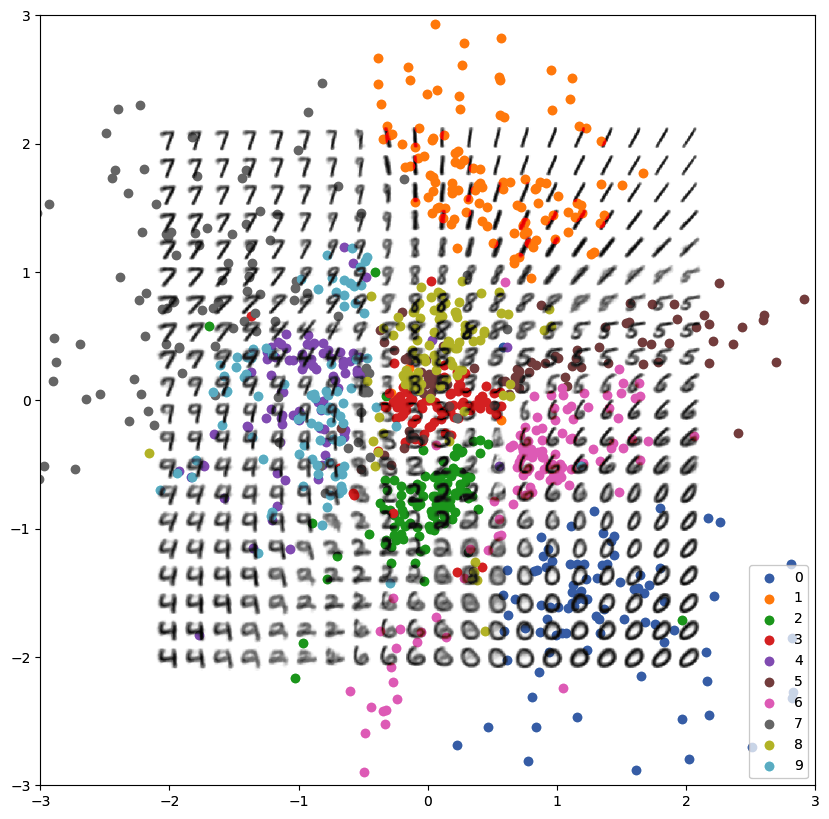
\includegraphics[width=140mm]{../img/mnist-manifold.png}
    \caption{Variational autoencoder learns to project 784-dimensional space of MNIST images down to only 2 dimensional space. We can see clusters of individual classes, forming high-density regions and being separated by low-density regions.}
    \label{fig:MnistManifold}
\end{figure}

\begin{figure}[p]
    \centering
    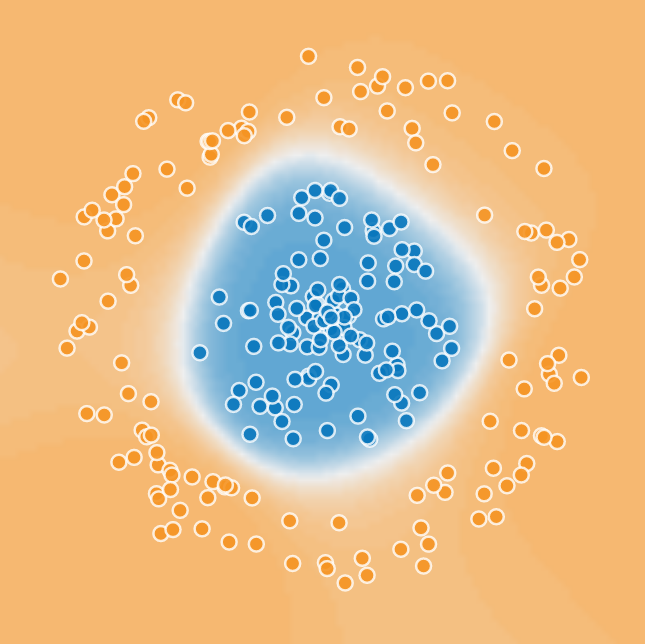
\includegraphics[width=50mm]{../img/decision-boundary.png}
    \caption{Visualization of a classification task, with the decision boundary visible in between the two classes (the while region). Image taken from the TensorFlow Playground at \url{https://playground.tensorflow.org/}.}
    \label{fig:DecisionBoundary}
\end{figure}

\qquad

The following text uses a terminology, that should be explained first. We will do that on an example:

Figure \ref{fig:MnistManifold} shows the latent space of a variational autoencoder trained on the MNIST dataset (\cite{VariationalAutoencoder}, \cite{Mnist}). This dataset contains grayscale images of handwritten digits, 28x28 pixels in size. In machine learning, the \emph{manifold hypothesis} states, that \emph{real-world high-dimensional datasets lie along low-dimensional manifolds inside that high-dimensional space}. The space of all 28x28 images is such a \textbf{high-dimensional space} (784 dimensions). Manifold, mathematically speaking, is a continuous, locally-eucleidian space (e.g.\@ a plane, sphere, 3D space, Möbius strip). The latent space of the autoencoder is a 2D plane (as seen in Figure \ref{fig:MnistManifold}) and it is the stated \textbf{low-dimensional manifold} containing all the data. The data points lie on this manifold, the model has only learned, how is this 2D manifold embeded in the 784-dimensional space. (Note that it is not the only manifold the data lies on, this is just the one discovered during training.)

The data points are not evenly scattered throughout the high-dimensional space. They are coalesced into groups called \textbf{clusters}. Points within these clsuters are located relatively close to each other and usually share the same class. This is a similar statement to saying that all digits 7 look alike. These clusters are clearly visible in the latent space (Fig. \ref{fig:MnistManifold}), where they form very distinct blobs. The space, where clusters sit, is refered to as \textbf{high-density regions} -- many items from the dataset are located here. Conversely, the space between clusters, where almost no data points are present, is refered to as \textbf{low-density regions}.

A classification task learns a function that assigns a label to each point of the input space. This label is discrete. We can color the input space according to the assigned label and that would produce regions, where all points have the same label. The place where these regions meet is called the \textbf{decision boundary}. A decision boundary can be seen in Figure \ref{fig:DecisionBoundary}. In a well-trained classifier for a well-defined classification problem, this decision boundary should lie in the described low-density regions.


\section{Assumptions}
\label{sec:SslAssumptions}

Before we start using semi-supervised methods, we should first understand assumptions that underpin them. These assumptions are mostly intuitive and are satisfied in almost all real-world problems, however stating them explicitly yields better understanding of these methods.

\begin{itemize}
    \item \textbf{The Smoothness Assumption.} \emph{If two points $x_1$, $x_2$ reside in a high-density region and are close together, then their corresponding outputs $y_1$, $y_2$ should also be close together.} For example, if we have a picture of digit 7, then small variations in its shape and color should still be interpreted as digit 7. The opposite statement also holds; if the two input points are separated by a low-density region, the outputs must be distant from each other. This assumption is primarily helpful in a classification task, not so much in a regression task.
    \item  \textbf{The Cluster Assumption.} \emph{If points are in the same cluster, they are likely to be of the same class.} This assumption connects the classification task to the smoothness assumption. It indirectly states, that the decision boundary is located in low-density regions, because otherwise it would cut a cluster in half, causing close points to fall to different classes (which is a violation of the assumption). This assumption can be used as a motivation for methods that push the decision boundary away from data points, into the low-density regions.
    \item \textbf{The Manifold Assumption.} \emph{The (high-dimensional) data lie (roughly) on a low-dimensional manifold.} The problem with high-dimensional data is that as the number of dimensions increases, the volume of the space grows exponentially. This means that most of the space is not covered by any data points in our dataset and that makes it difficult to learn to classify. This assumption states, that our data points actually lie on a small subspace (manifold) of the entire space and that a projection can be learned, that maps this manifold onto a low-dimensional space. Learning the classification task for this low-dimensional space should be much easier.
\end{itemize}


\section{Methods}
\label{sec:SslMethods}

The following section lists major SSL methods. These methods are often directly based on previously stated assumptions and are not mutually exclusive, in fact most of them can be used simultanously as so-called holistic methods. These are, however, not covered in this chapter.


\subsection{Consistency Regularization}

The core idea of this method is that a small neighborhood of each datapoint should have the same label as that datapoint. This idea follows directly from the cluster assumption. In this method, we train the model to minimze distance between a known datapoint $x$ and a perturbed datapoint $\hat{x}$. This training is performed in addition to the usual supervised training. This method does not rely on the corresponding label $y$, instead it trains to minimize the distance between $f(x)$ and $f(\hat{x})$. This lets us utilize all unlabeled data points as well.

The method can be seen as an extension of supervised learning. In supervised learning, we train on individual points and learn the overall shape from them. Here, we train on small neighbourhoods, which makes sure the decision boundary will not come close to any individual datapoint. Further utilization of unlabeled data points in the proximity of labeled data points should force the decision boundary even further away, into low-density regions (\cite{SslTechnicalReport}).

\begin{figure}[ht]
    \centering
    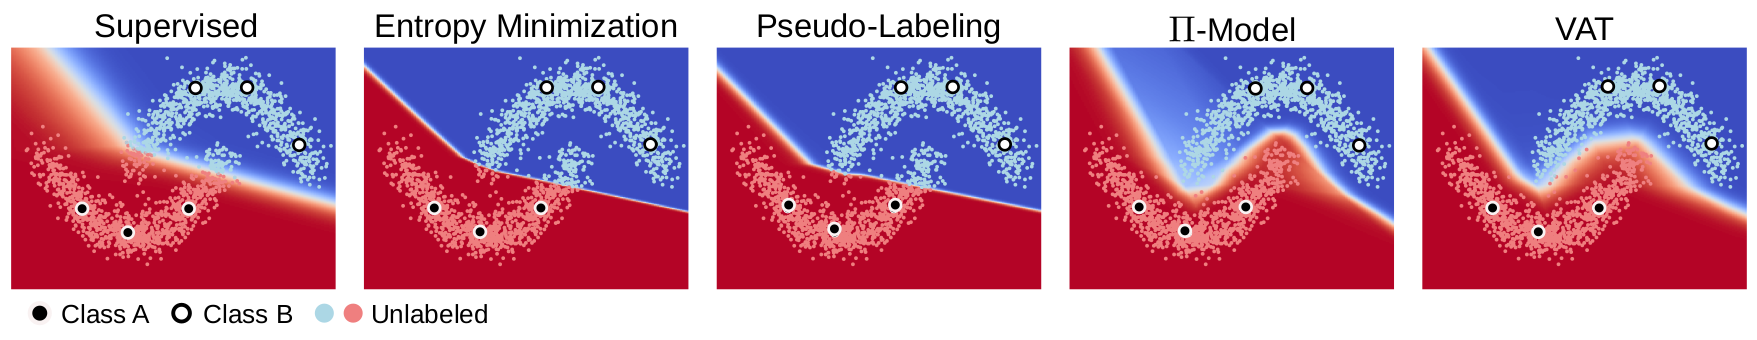
\includegraphics[width=145mm]{../img/ssl-toy.png}
    \caption{SSL toy example -- the \emph{two moons} dataset with three labeled examples for each class. $\Pi$-model and VAT are both consistency regularization techniques. The image is taken from \cite{SemisupervisedOverview}.}
    \label{fig:SslToy}
\end{figure}


\subsection{Proxy-label Methods}

This is a set of methods, that train a supervised model on the labeled data and then use it to label portion of the unlabeled data. These methods are also called \emph{bootstrapping}. To distinguish these later-added labels, they are called \emph{pseudo-labels}.

One of these methods is \emph{self-training}. In self-training, labeled data is used to train a supervised classification model. This model is then used to classify all unlabeled data points and since its output is a softmax layer, we can not only pick the most likely class, but also measure the confidence in that class. We define a threshold $\tau$ and only assign pseudo-labels to data points above this threshold. This process can be repeated, until a stopping condition is met (e.g.\@ there are no more unlabeled points with confidence above $\tau$). The main problem of this method is the inability to correct mistakes made during the labeling step.

\emph{Pseudo-labeling} is a similar method, where the unlabeled data points are also assigned pseudo-labels. In this case, these pseudo-labels are treated as trainable parameters, similar to model parameters, and are optimized together with the model during training. The difficult part is designing a good loss function for pseudo-labels, because applying this method naively causes the pseudo-labels to overfit, due to so-called confirmation bias.

Self-training has been used for semantic segmentation in the work of \cite{SelfTrainingSegmentation}.


\subsection{Graph-based Methods}

These methods frame the problem in the language of graphs (\cite{SslTechnicalReport}). Data points are represented as vertices of a graph and weighted edges are present between pairs of vertices, where the weight corresponds to some similarity between the two points. The labeling task can be viewed as a propagation of information along edges of the graph.

This propagation resembles proxy-label methods, however due to the graph framing, we can consider things like vertex neighbourhood and its impact on the examined node, or we can leverage algebraic structures like adjacency matrix.

A different set of graph methods aims to learn data point embeddings, which preserve the structure of the input graph. The goal is to represent each vertex (data point) as a low-dimensional vector, where a simple similarity function (e.g.\@ inner product) can be used. This again resembles deep learning techniques, such as autoencoding (see Figure \ref{fig:MnistManifold}), however here, methods derived from graph theory are used to produce these embeddings (e.g.\@ Laplacian Eigenmaps or Locally Linear Embeddings).


\subsection{Entropy Minimization}
\label{sec:EntropyMinimization}

Consistency regularization methods attempt to push the decision boundary away from clusters and into the low-density regions by stabilizing the model output in a neighborhood around each data point. Entropy minimization is a different technique that attempts to do the same thing. In entropy minimization, we penalize the model for being unsure about its predictions. Low-confidence predictions are predictions with more than one class having non-zero probability. Such probability distributions have higher entropy than one-hot distributions. By adding a loss term that minimizes entropy of predictions during training, we can make areas around datapoints more stable (\cite{EntropyMinimization}). This method can not, however, be used alone for high-capacity models (deep neural networks), as it causes the training to overfit. Instead, it may be used as a supplementing technique to another SSL technique.


\section{Generative Methods}
\label{sec:GenerativeSslMethods}

Generative semi-supervised learning leverages generative models for the classification task. A generative model learns to describe the distribution of data $p(x)$. The assumption here is that this understanding helps the model with the classification task $p(y|x)$. Generative SSL can be viewed either as an extension of supervised learning (classification with the addition of $p(x)$ modeling), or as an extension of unsupervised learning (modeling, extended by label information).


\subsection{Variational Autoencoders}

A variational autoencoder (VAE) (\cite{VariationalAutoencoder}) is a model that attempts to learn a mapping between the input space and a smaller latent space. The latent space is also required to roughly follow a unit gaussian distribution, which causes the space to be filled and smooth, such that sampling any point of this space yields a reasonable corresponding data point. Moreover, the model architecture forces clusters of similar data points to occupy roughly gaussian-shaped regions in the latent space. A visualization of this latent space can be seen in Figure \ref{fig:MnistManifold}. The variational autoencoder consists of an encoder and a decoder. The encoder learns the mapping from the input space to the latent space and the decoder learns the inverse mapping. The decoder is then considered as the generative model, as it can generate a reasonable data point for an arbitrary latent space point. Input data points are typically denoted $x$ and the latent vectors are denoted $z$.

\cite{KingmaSslVae} used variational autoencoders in a semi-supervised setting. They propose three ways of extending VAEs:

\paragraph*{M1 Model}
First, an unsupervised VAE model is pre-trained using all available labeled and unlabeled samples. The goal is to learn a low-dimensional latent space and then transform all data points to this space (create embeddings). After this, a supervised classifier is trained on these embeddings using only the labeled portion of the data. This setup leverages the manifold assumption and the assumption that learning classification in a low-dimensional space is easier than in a high-dimensional space. Also, since the variational autoencoder forces the creation of gaussian-shaped clusters in the latent space, the classifier has an easier job separating these clusters.

\paragraph*{M2 Model}
In the previous setup, labels $y$ were ignored when training the autoencoder. Here, the latent vector $z$ is extended by an additional vector $y$. This vector will be set to the label, if the label is known and will be left unconstrained for unlabeled data. We can view this as splitting the original latent vector $z$ into two parts, one being left free to be trained as usual, and the second (categorical) part being sometimes trained to match the label $y$ of the learned datapoint $x$. If the label is not known, this part is trained in the unsupervised mode only, like the original latent variable $z$. When the training finishes, the encoder can be immediately used as a classifier, by interpreting the latent vector $y$ as the output label. The two parts of the latent representation ($z$ and $y$) can be interpreted as style and content embddings respectively.

\paragraph*{M1 + M2 Model}
The last setup involves training the model M1 in the unsupervised way and then training the model M2 in semi-sueprvised way on embeddings produced by M1. It can be viewed as the M2 model, utilizing dimensionality reduction by M1. This stacked setup yields the best results.


\subsection{Adversarial Autoencoders}

A newer article by \cite{AdversarialAutoencoders} introduces an architecture, called an Adversarial Autoencoder (AAE). The architecture is in many ways similar to the variational autoencoder, but it differs in the way it regularizes its latent space. Whereas a VAE uses KL-divergence loss to force the latent space into a gaussian distribution, an AAE uses a discriminator network (inspired by generative adversarial networks). This architecture can be used and extended in similar ways to the M1 and M2 models and yields even better results for tasks, such as semi-supervised classification, unsupervised clustering and style-content disentangling.

\begin{figure}[ht]
    \centering
    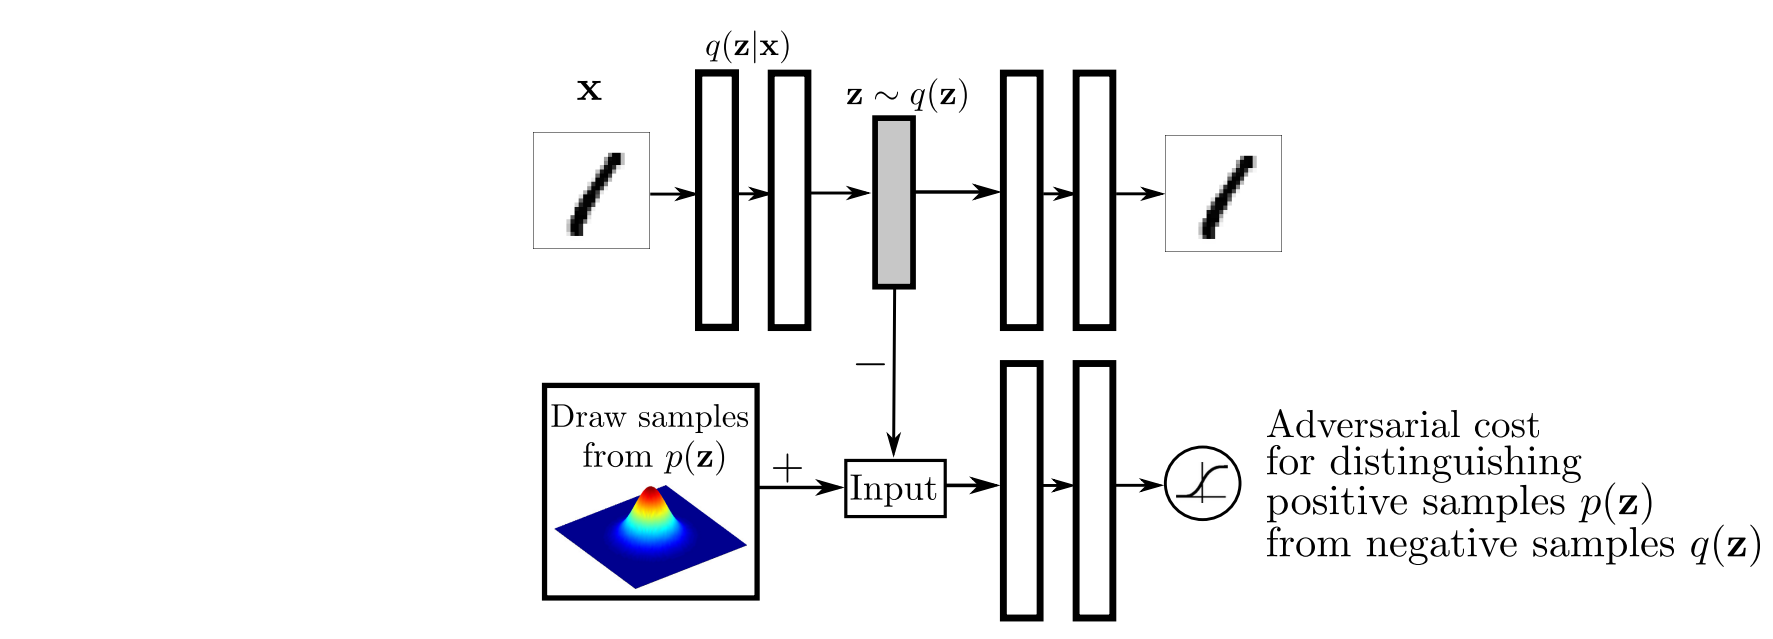
\includegraphics[width=145mm]{../img/aae.png}
    \caption{Architecture of an adversarial autoencoder. The top two networks form a typical autoencoder with the embedding vector in the middle. The bottom model is a discriminator, forcing the encoder to produce embeddings matching the distribution $p(\mathbf{z})$. The image is taken from \cite{AdversarialAutoencoders}.}
    \label{fig:AaeArchitecture}
\end{figure}


\subsection{Generative Adversarial Networks}

Generative adversarial network (GAN) is a generative architecture consisting of two parts: a generator and a discriminator (\cite{GAN}). They are trained together in an alternating fashion, where the generator is trained to produce realistic-looking data (to fool the discriminator) and the discriminator is trained to distinguish this generated data from the real-world data. The tension between these two models causes both of them to get increasingly better and the generator ends up producing well-looking synthetic samples. Input to the generator is a latent vector $z$, drawn from a prior distribution (e.g.\@ a gaussian). The generator uses this vector as a seed for the generation. The discriminator outputs a single value, interpreted as the probability of the shown sample being real or generated.

\paragraph*{CatGAN}
Categorical generative adversarial networks (CatGAN) replace the discriminator with a classifier (\cite{CatGAN}). The output of this classifier is a softmax layer with C neurons. The discriminative task is transformed onto the classifier by considering its certainty of prediction. In the section on entropy minimization (Section \ref{sec:EntropyMinimization}), we described how certainty of prediction is related to entropy of the predicted distribution, and also how the entropy can be minimized (or maximized) to force the model to be certain (uncertain). In the unsupervised mode, the classifier is trained to output one (any) of the classes for real data points with maximum certainty -- to recognize real samples. The generator is then trained to confuse the classifier to produce uncertain predictions (uniform distribution).

In SSL, the classifier is trained to produce confident predictions of any class for unlabeled data and confident predictions of known class for labeled data. The supervised loss is a categorical cross-entropy (like in a typical classification setup) and the unsupervised loss is an entropy minimization loss (to force confident predictions of any class).

\paragraph*{DCGAN, SGAN}
Deep Convolutional GANs attempt to learn intermediate representations by training convolutional GANs on unlabeled data (\cite{DCGAN}). Parts of the generator and discriminator are then re-used as feature extractors for supervised classification task. Semi-supervised GANs (SGAN) address and fix issues with DCGAN, such as the fact that the classifier is trained after the GAN has finished training (\cite{SGAN}). SGAN is able to train the generator and classifier simultaneously, substantially improving classification performance.

\paragraph*{BiGAN}
In a typical GAN, the latent variable $z$ is only used as a seed for the generator and the generator acts as function $G: Z \rightarrow X$. In a variational autoencoder, there exists a full bijection between spaces $X$ and $Z$. BiGANs extend the basic GAN framework by adding an encoder, that acts as a mapping $E: X \rightarrow Z$ (\cite{BiGAN}). This gives us access to the latent vector $z$ of an existing real-world sample $x$. The discriminator is extended to have access to both the data points and the latent points, and so it discriminates between pairs of $(x, E(x))$ and $(G(z), z)$. BiGAN therefore serves a similar role to a variational autoencoder and can be extended for use in semi-supervised learning.


\section{Related Methods}
\label{sec:RelatedSslMethods}

\paragraph*{Transfer Learning} In transfer learning, the goal is to utilize the knowledge about one problem to solve another different but related problem. For example, utilizing layers of an already trained network (e.g.\@ an autoencoder) as feature extractors for a different task (e.g.\@ classification) is an example of transfer learning.

\paragraph*{Domain Adaptation} In the previous example of transfer learning, the two tasks have different feature space. Domain adaptation is a subset of transfer learning where both tasks have the same feature space, but different data distribution. For example, training a classifier of handwritten digits on augmented printed digits (handwritten and printed digit images are both images, just with different distributions). Semi-supervised learning differs from domain adaptation in that both problems have the same data distribution (the training and test data come from the same process).

\paragraph*{Muti-task Learning} Multi-task learning is the process of training one model to solve two different tasks simultaneously. By having one model learn both tasks, the model can share intermediate representations for both of them, achieving better performance, than by having a dedicated model for each task.
